\begin{figure}[h]
    \centering
    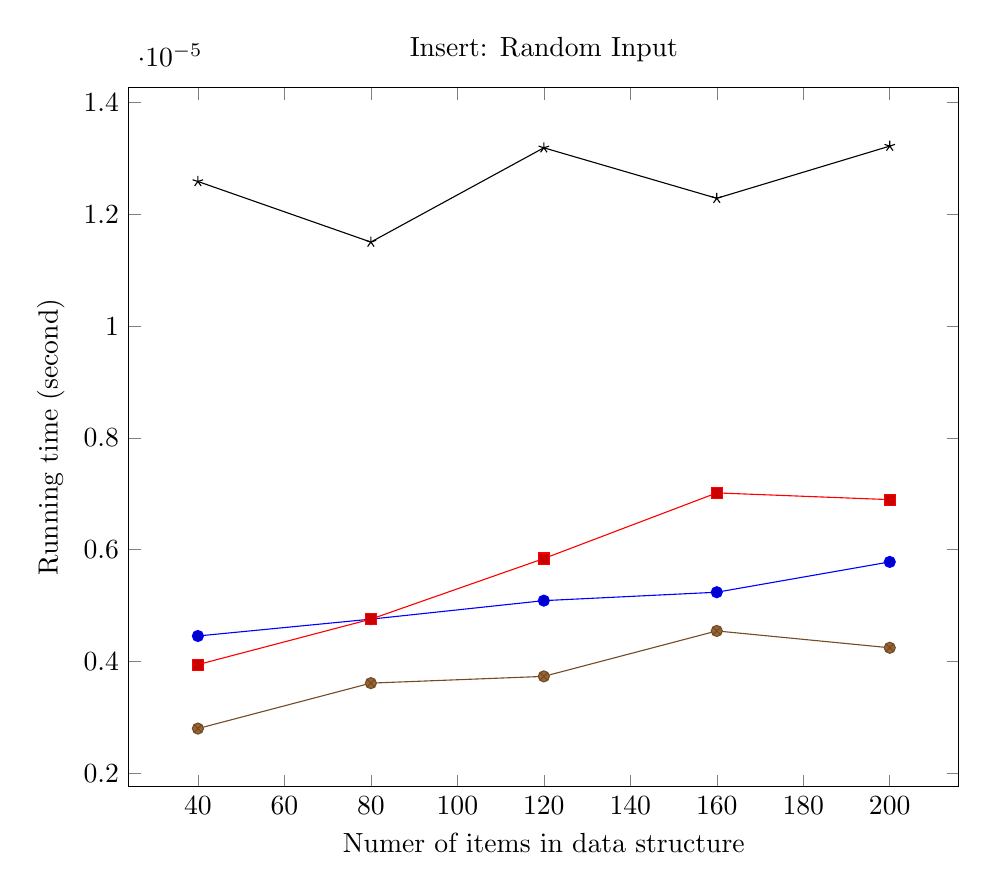
\begin{tikzpicture}
        \begin{axis}[
            xlabel={Numer of items in data structure},
            ylabel={Running time (second)},
            title={Insert: Random Input},
            width=\textwidth
        ]
		\addplot coordinates {
			(200, 5.782566465632744e-06)
			(160, 5.240450859479717e-06)
			(120, 5.0898631911044935e-06)
			(80, 4.758570320675948e-06)
			(40, 4.4573949839255e-06)
		};
		\addplot coordinates {
			(200, 6.896915211612731e-06)
			(160, 7.0173853463140205e-06)
			(120, 5.842801532982e-06)
			(80, 4.758570320677335e-06)
			(40, 3.945396911446408e-06)
		};
		\addplot coordinates {
			(200, 4.246572248198244e-06)
			(160, 4.547747584950079e-06)
			(120, 3.73457417572054e-06)
			(80, 3.6141040410192505e-06)
			(40, 2.800930631789711e-06)
		};
		\addplot coordinates {
			(200, 1.32215972833985e-05)
			(160, 1.228795373946906e-05)
			(120, 1.3191479749723178e-05)
			(80, 1.1504897863913454e-05)
			(40, 1.2589129076219508e-05)
		};
        \legend{}
        \end{axis}
    \end{tikzpicture}
    \caption{Average of 0 operations, benchmarked every 0, starting at 0.}
\end{figure}